\documentclass[12pt]{article}
\usepackage{amsmath}
\usepackage{amssymb}
\usepackage{geometry}
\usepackage{enumerate}
\usepackage{natbib}
\usepackage{float}%稳定图片位置
\usepackage{graphicx}%画图
\usepackage[english]{babel}
\usepackage{a4wide}
\usepackage{indentfirst}%缩进
\usepackage{enumerate}%加序号
\usepackage{multirow}%合并行
\title{\large UM-SJTU JOINT INSTITUTE\\PHYSICS LABORATORY\\(VP141)\\\ \\\ \\\ \\\ \\\ \\\ \\\ \\\ \\\ \\\ \\\
LABORATORY REPORT\\\ \\\ EXERCISE 4\\\  MEASUREMENT OF THE SPEED OF SOUND \\\ \\\ \\\ \\\ \\\ }
\author{Name: Pan Chongdan\\ID: 516370910121\\Partner: Yang Ruiming\\ID:516370910127\\Group: 16}
\date{Date: \today}

\begin{document}
\maketitle
\newpage
\section{Objectives}
In the exercise, I'll learn various methods to measure the speed of sound in air: the resonance method, the phase comparison method and the time difference method. What's more, I'll become familiar with the successive difference method in measurement data processing.
\section{Theoretical Background}
\subsection{Basic Quantitative Characteristics of Sound Waves} 
Sound is a mechanical wave that propagates through a compressible medium. It is a
longitudinal wave because the direction of vibrations of the medium is the same as the direction of propagation. The frequency of sound perceptible to a human ear ranges from about 20 Hz to 20 000 Hz. Sound with the frequency higher than 20000 Hz is called \emph{ultrasound}. In this experiment an ultrasonic wave is chosen as the signal source, because its wavelength is short enough to measure the speed of sound precisely.
\par The phase speed $v$, the frequency $f$ and the length $\lambda$ of a wave are related by the formula
\begin{equation}
v=\lambda f.
\end{equation}
For motion with constant speed $v$ along a straight line, we have
\begin{equation}
v=\frac{L}{t},
\end{equation}
where $L$ is the distance travelled over time $t$. Hence, if the distance and the time a wave front travels is known, the phase speed may be found.
\subsection{Measurement Method}
The experimental setup consists of a signal source, two piezoelectric transducers $S_1$ and $S_2$, and oscilloscope arranged as shown in Figure 1.
\begin{figure}[H]
\centering
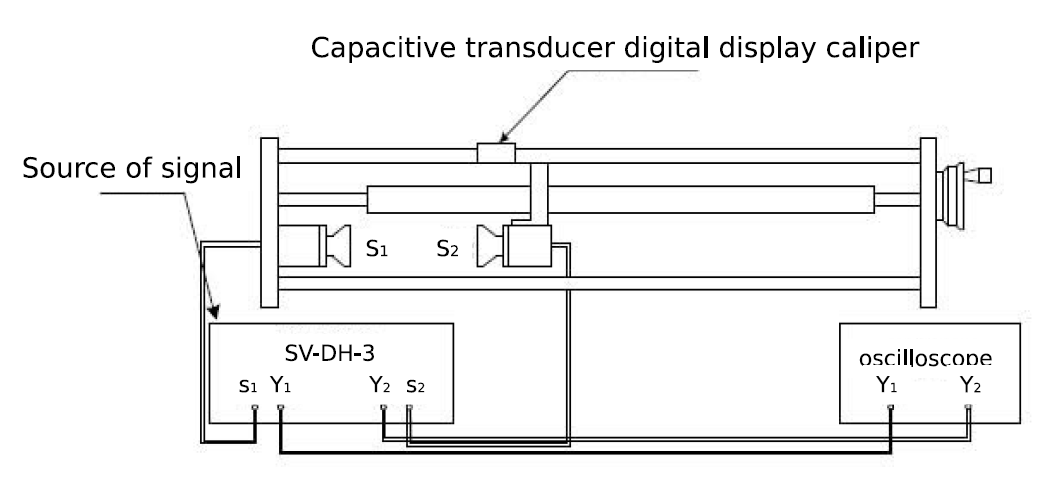
\includegraphics[scale=0.3]{P1.jpg}
\caption{Measurement setup}
\end{figure}
\subsubsection{Resonance Method}
The elements $S_1$ and $S_2$ are the wave source and the receiver and reactors, respectively, placed a distance $L$ from each other. If they are arranged parallel to each other, the sound wave is reacted. If
\begin{equation}
L=n\frac{\lambda}{2}
\end{equation}
where n=1,2,$\cdots$ the distance is a multiple of half-wavelength, standing waves will form, and maximum speed will be observed in the oscillograph (Figure 2). The distance between two successive maxima $(L_{i+1}-L_i)$ is always $\lambda /2$. After the position corresponding to each maximum is measured, it is easy to find the wavelength and then the speed of sound by using Eq. (1). The frequency $f$ is displayed directly on the signal generator.
\begin{figure}[H]
\centering
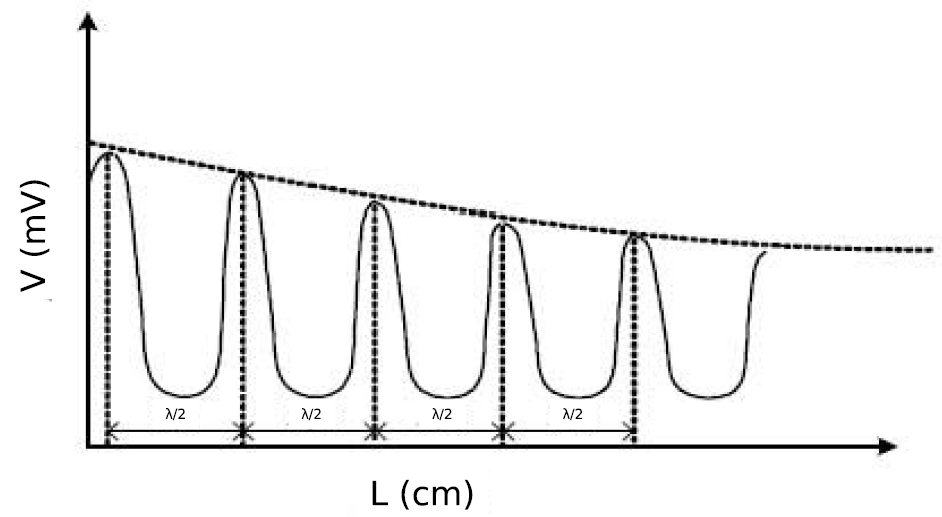
\includegraphics[scale=0.5]{P2.jpg}
\caption{Relationship between the signal voltage and the distance between the transducers.}
\end{figure}
\subsubsection{Phase-comparison Method}
If the phase of the wave at two points on the wave propagation direction is equal, then the distance between these points $L$ has to be a multiple of the wavelength, for example:$$L=n\lambda,$$where n=1,2,$\cdots$ The experimental setup for the phase comparison method is the same as in the previous method (Figure 1). Lissajous figures are used to identify the values of $L$. Lissajous figures (or Lissajous curves) are trajectories of a particle that moves in a plane so that it moves in a harmonic motion independently along two perpendicular directions (for example the axes $x$ and $y$ of a Cartesian coordinate system), so that $\textbf{r}(t)=(A_x cos(\omega_xt+\phi_x),A_y cos(\omega_yt + \phi_y)).$When the two superimposed harmonic motions have
identical frequency $\omega_x=\omega_y$ and phase difference $|\phi_x-\phi_y|= n\pi$, where n=0,1,2,$\cdots$ the Lissajous figure will show as a straight line. For other values of the phase difference the figures will have an elliptical shape.
\subsubsection{Time-difference Method}
The successive difference method is an effective method to increase the accuracy of
the average value calculated from a series of measurement data. In this experiment, the usual method of calculating the average value, illustrated by the formula
\begin{equation}
\frac{\bar{\lambda}}{2}=\frac{[(L_1-L_0)+(L_2-L_1)+\cdots+(L_n-L_{n_1})]}{n}=\frac{L_n-L_0}{n}
\end{equation}
will be modified, because as equation (4) shows, the average value of the wavelength is determined only by the first and the last value, $L_0$ and $L_n$.
\par A modification of the formula by rearranging terms as
\begin{equation}
n\frac{\bar{\lambda}}{2}=\frac{\sum_{i=1}^n(L_{n+i}-L_i)}{n},
\end{equation}
produces more accurate results, as each value contributes to the final result.
\section{Apparatus}
\begin{enumerate}
\item In the exercise, the most important apparatus I used is Oscilloscope. The oscilloscope can draw the figure of the wave and Lissajous figures for me to calculate the speed and wavelength of sound.
\begin{figure}[H]
\centering
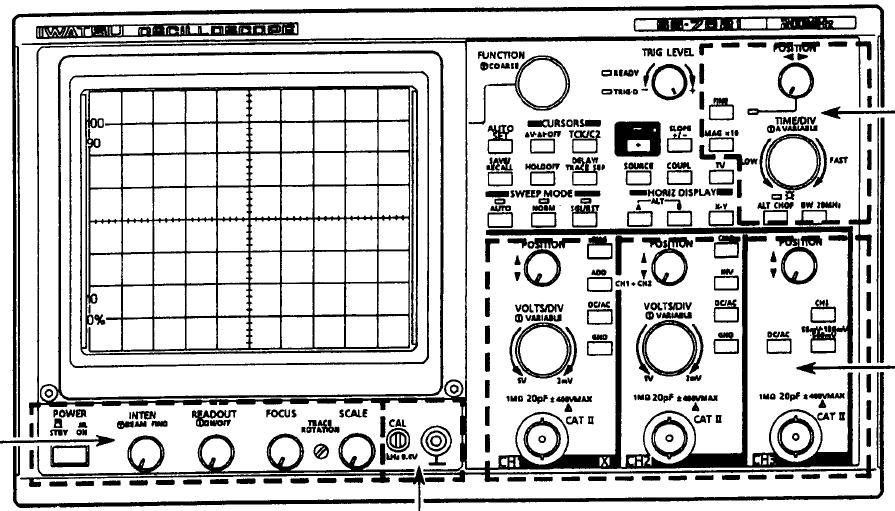
\includegraphics[scale=0.5]{P4.jpg}
\caption{Oscilloscope}
\end{figure}
\item The second apparatus is the signal sources, which keeps the frequency of sound is 34500 Hz.
\item I also used two piezoelectric transducers in water and air respectively to read and adjust the distance between the transducers.
\item An thermometer with resolution is $1^oC$ is used to measure the temperature in the lab.
\end{enumerate}
\section{Measurement Procedure}
\subsection{Resonance Method}
\begin{enumerate}
\item Set the initial distance between $S_1$ and $S_2$ at about 1 cm.
\item Turn on the signal source and the oscilloscope. Then set the following options on the panel of the signal source
\begin{enumerate}[(1)]
\item Choose \emph{Continuous} wave for \emph{Method}.
\item Adjust \emph{Signal Strength} until a 10 V peak voltage is observed on the oscilloscope.
\item Adjust \emph{Signal Frequency} between 34.5 kHz and 40 kHz until the peak-to-peak voltage reaches its maximum. Record the frequency.
\end{enumerate}
\item Increase $L$ gradually by moving $S_2$, and observe the output voltage of $S_2$ on the oscilloscope. Record the position of $S_2$ as $L_2$ when the output voltage reaches an maximum.
\item Repeat step 3 to record 20 values of $L_2$ and calculate $v$.
\end{enumerate}
\subsection{Phase-comparison Method}
\begin{enumerate}
\item Use Lissajous figures to observe the phase difference between the transmitted and the received signals. Move $S_2$ and record the position when the Lissajous figure
becomes a straight line with the same slope.
\item Repeat step 1 to collect 12 sets of data. Use the successive difference method to process the data and calculate $v$.
\end{enumerate}
\subsection{Time-difference Method (Air)}
Since the pulse wave causes damped oscillations at the receiver, there will be significant interference if $S_1$ and $S_2$ resonate. The resonance can be observed on the oscilloscope.
\begin{enumerate}
\item Choose \emph{Pulse Wave} for \emph{Method} on the panel of the signal source.
\item Adjust the frequency to 25 Hz and the width to 500 $\mu$s.
\item Record the distance $L_1$ and the time $t_1$.
\item Move $S_2$ to another position and repeat step 3. Record $L_i$ and $t_i,i=2,3,4\cdots$
\item Repeat step 4 to collect 12 pairs of $L_i$ and $t_i$. Plot the $L_i=L_i(t_i)$ graph and use computer software to find a linear fit to the data. The slope of the line is the speed $v$.
\end{enumerate}
\subsection{Time-difference Method in (Liquid)}
\begin{enumerate}
\item Change the medium to water.
\item Adjust the frequency to 100 Hz and the width to 500 $\mu$s.
\item Use the cursor function of the oscilloscope to measure the time and the distance
between the the starting points of neighbouring periods. Record 12 pairs of data and
calculate $v_{water}$.
\end{enumerate}
\section{Calculation and Results}
\subsection{Measurement Data}
\subsubsection{Constant Physical Quantity in Lab}
The frequency of the sound wave $f$=34500[Hz]
\par Temperature T= [29$^o$C]$\pm$[$1^o$C]
\subsubsection{Data for the Resonance Method}
\begin{table}[H]
\centering
\begin{tabular}{|c|c|c|c|c|c|}
\hline
\multicolumn{2}{|c|}{$L_i$[mm] $\pm$ 0.01[mm]} & \multicolumn{2}{c|}{$L_i$[mm] $\pm$ 0.01[mm]} & \multicolumn{2}{c|}{$L_{10+i}-L_i$[mm]} \\ \hline
1           &10.72          & 11         &61.32          & 1          &50.60          \\ \hline
2           &15.73          & 12         &66.41          & 2          &50.68          \\ \hline
3           &20.05          & 13         &71.61          & 3          &51.56          \\ \hline
4           &25.22          & 14         &76.72          & 4          &51.50          \\ \hline
5           &30.36          & 15         &81.91          & 5          &51.55          \\ \hline
6           &35.59          & 16         &87.05          & 6          &51.46          \\ \hline
7           &40.82          & 17         &92.14          & 7          &51.32          \\ \hline
8           &45.98          & 18         &97.07          & 8          &51.09          \\ \hline
9           &51.01          & 19         &102.22          & 9          &51.21        \\ \hline
10          &56.11          & 20         &107.37          & 10         &51.26          \\ \hline
\end{tabular}
\caption{Data table for the resonance method}
\end{table}
\subsubsection{Data for the Phase Comparison Method}
\begin{table}[H]
\centering
\begin{tabular}{|c|c|c|c|c|c|}
\hline
\multicolumn{2}{|c|}{$L_i$[mm] $\pm$ 0.01[mm]} & \multicolumn{2}{c|}{$L_i$[mm] $\pm$ 0.01[mm]} & \multicolumn{2}{c|}{$L_{6+i}-L_i$[mm]} \\ \hline
1          &11.44           & 7          &43.80          & 1          &32.36          \\ \hline
2          &16.90           & 8          &49.64          & 2          &32.74          \\ \hline
3          &22.32           & 9          &54.75          & 3          &32.43          \\ \hline
4          &27.85           & 10         &60.20          & 4          &32.35          \\ \hline
5          &33.34           & 11         &65.51          & 5          &32.17          \\ \hline
6          &38.61           & 12         &71.05          & 6          &32.44          \\ \hline
\end{tabular}
\caption{Data table for the phase comparison method}
\end{table}
\subsubsection{Data for the Time Difference Method (Liquid)}
\begin{table}[H]
\centering
\begin{tabular}{|c|c|c|}
\hline
   & $t_i$[$\mu$s] $\pm$ 0.2[$\mu$s] & $L_i$[mm] $\pm$ 0.01[mm]  \\ \hline
1  &82.8  &110.00  \\ \hline
2  &89.4  &120.36  \\ \hline
3  &96.0  &130.31  \\ \hline
4  &102.8  &140.25  \\ \hline
5  &109.2  &150.15  \\ \hline
6  &116.0  &160.13  \\ \hline
7  &122.6  &170.13  \\ \hline
8  &129.4  &180.09  \\ \hline
9  &136.0  &190.22  \\ \hline
10 &142.8  &200.05  \\ \hline
11 &149.2  &210.30  \\ \hline
12 &156.2  &220.42  \\ \hline
\end{tabular}
\caption{Data table for the time difference method (liquid)}
\end{table}
\subsection{Calculations}
\subsection{Calculation for Resonance Method}
$$\bar{L}=\frac{\sum_{i=1}^{10}L_{10+i}-L_i}{10}=51.223[mm]$$
According to equation (3),$$L=10\times\frac{\lambda}{2}$$
$$\lambda=\frac{\bar{L}}{5}=\frac{51.223}{5}=10.245[mm]$$
$$v=\lambda f=10.245\times34500\times10^{-3}=353.439[m/s]$$
\subsection{Calculation for the Phase Comparison Method}
$$\bar{L}=\frac{\sum_{i=1}^{6}L_{10+i}-L_i}{10}=32.415[mm]$$
According to $L=n\lambda$, $$\lambda=\frac{L}{3}$$
$$\lambda=\frac{\bar{L}}{3}=\frac{32.415}{3}=10.805[mm]$$
$$v=\lambda f=10.805\times34500\times10^{-3}=372.77[m/s]$$
\subsection{Calculation for the Time Difference Method (Liquid)}
According to equation (2),$v=\frac{L}{t}$, I can use origin to draw linear fit diagram to get $v_{water}$, which is the slope of L vs. t diagram
\begin{figure}[H]
\centering
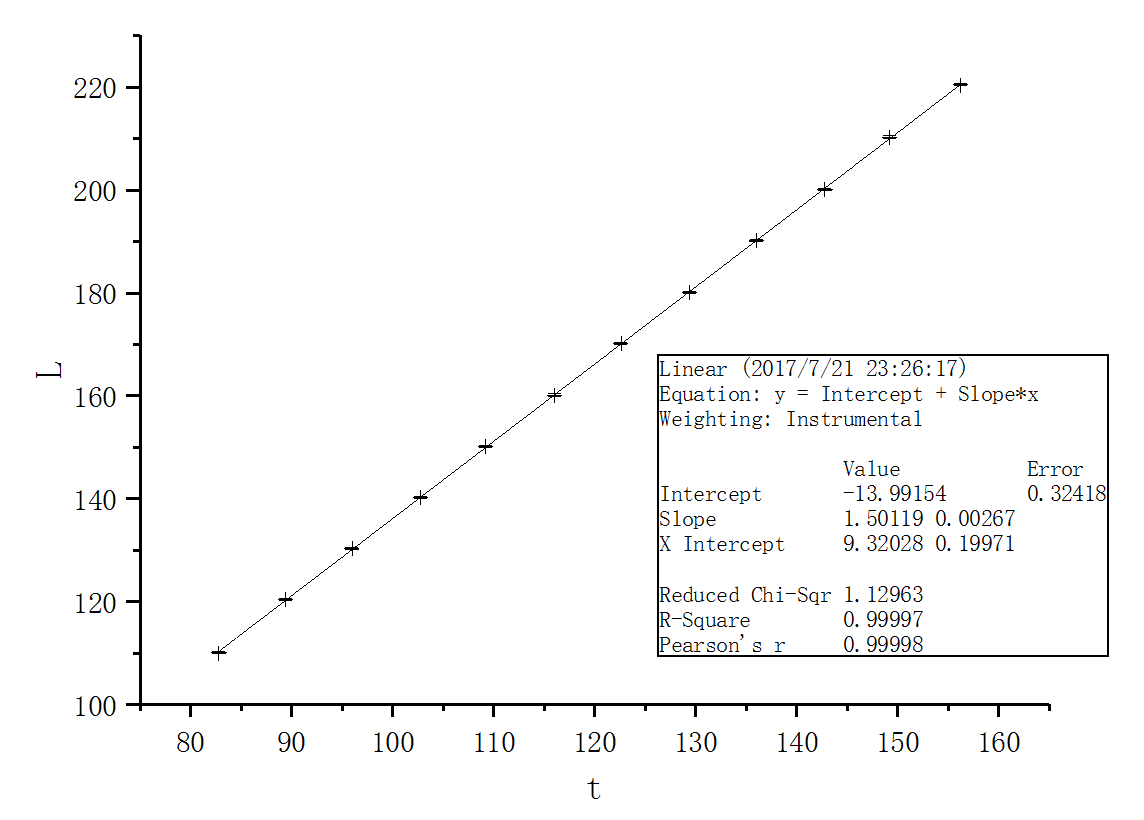
\includegraphics[scale=0.5]{P3.jpg}
\caption{Linear fit diagram for time difference method (liquid)}
\end{figure}
So $v_{water}=1.501[mm/\mu s]=1501[m/s]$
\section{Measurement Uncertainty Analysis}
\subsection{Measurement Uncertainty for Resonance Method}
$$u_{\bigtriangleup L}=\sqrt{2(u_L)^2}=\sqrt{2\times(0.01)^2}=0.0141[mm]$$
$$u_{\bar{L}}=\sqrt{10\times(\frac{u_{\bigtriangleup L}}{10})^2}=4.47\times10^{-3}[mm]$$
$$u_{\lambda}=\frac{u_{\bar{L}}}{5}=8.94\times10^{-4}[mm]$$
$$u_v=u_{\lambda}f=\frac{8.94\times10^{-4}\times34500}{1000}=3.09\times10^{-2}[m/s]$$
$$u_r=\frac{u_v}{v}\times100\%=\frac{3.09\times10^{-2}}{353.44}\times100\%=0.01\%$$
\subsection{Measurement Uncertainty for the Phase Comparison Method}
$$u_{\bigtriangleup L}=\sqrt{2(u_L)^2}=\sqrt{2\times(0.01)^2}=0.0141[mm]$$
$$u_{\bar{L}}=\sqrt{6\times(\frac{u_{\bigtriangleup L}}{6})^2}=5.77\times10^{-3}[mm]$$
$$u_{\lambda}=\frac{u_{\bar{L}}}{3}=1.92\times10^{-3}[mm]$$
$$u_v=u_{\lambda}f=\frac{1.92\times10^{-3}\times34500}{1000}=6.64\times10^{-2}[m/s]$$
$$u_r=\frac{u_v}{v}\times100\%=\frac{6.64\times10^{-2}}{372.77}\times100\%=0.02\%$$
\subsection{Measurement Uncertainty for the Time Difference Method (Liquid)}
According to the linear fit diagram, the uncertainty $u_{water}=2.67[m/s]$ 
$$u_r=\frac{u_v}{v}\times100\%=\frac{2.67}{1501}\times100\%=0.18\%$$
\section{Conclusion and Discussion}
\subsection{Conclusion}
In the exercise, I used three methods to measure the speed of sound in air and water.
\begin{table}[H]
\centering
\begin{tabular}{|c|c|c|c|}
\hline
   & v[m/s] & $u_v$[m/s] &$u_r[\%$]  \\ \hline
$v_{resonance}$  &353.44  &$3.09\times10^{-2}$&0.01  \\ \hline
$v_{phase}$  &372.77  &$6.64\times10^{-2}$&0.02  \\ \hline
$v_{water}$  &1501  &$2.67$&0.18  \\ \hline
\end{tabular}
\caption{Measured speed of sound}
\end{table}
Through the exercise, I have a rough idea about what piezoelectric transducers and oscilloscope is and how to use them. The exercise also enrich my knowledge about wave and the speed of sound in different medium. I also know how to use successive difference method in measurement data processing.
\subsection{Discussion}
\subsubsection{Error Analysis}
\begin{enumerate}
\item The relative uncertainty in the third measurement is much bigger than other two. Although its medium is different from the others, I think it's the time different method that results in the error.
\item In the second measurement, I should have measure $L_{6+i}-L_i$ as 6 times wavelength. However, since I recorded the data as soon as the Lissajous figures becomes a line, the phase difference is actually $\phi$ while in the procedure its should be 2$\phi$, which means I should record the data every two lines. As a result, my $L_{6+i}-L_i$ is 3 times wavelength, and I change n from 6 to 3 in my calculations. Although my uncertainty in this measurement is not very big, but such mistakes may cause errors.
\end{enumerate}
\subsection{Questions for Considersion}
\subsubsection{Why Measure T?}
In the air, when the temperature is higher, the speed of sound will be bigger. Since sound wave propagate through the vibration of air molecules, the speed will be bigger when the vibration is more violent, which is caused by higher temperature. This can also affect the speed in liquid/
\subsubsection{Why not Use Time Difference Method in Air?}
The density of air is not as uniform as in liquid, and the drag force is also not uniformly distributed in air. As a result, the speed of sound may be changeable so the time difference may be not accurate enough.  
\subsubsection{Why $L_1>100mm$ in Time difference Method?}
I think the wavelength is bigger than 100mm so the wave can't be formed when $l_1>100mm$
\section{Data Sheet}
Data sheet is attach to the report
\section{Reference}
\begin{enumerate}[-]
\item Young, H.D., Freedman R.A. University Physics. Chapter 9,10.
\item Qin Tian, Zeng Ming, Zhao Xijian, Krzyzosiak,M. Lab Manual of Exercise 4.
\item Qin Tian, Zeng Ming, Zhao Xijian, Krzyzosiak,M. Handbook-Uncertainty Analysis.
\end{enumerate}
\end{document}